\documentclass[11pt,letterpaper]{article}
\usepackage[margin=1in]{geometry}
\usepackage[T1]{fontenc}
\usepackage{lmodern,microtype}
\usepackage{amsmath,amssymb,booktabs,array,longtable,float}
\usepackage{xcolor,hyperref}
\usepackage{tikz}
\usepackage{graphicx}
\graphicspath{{paper/figures/}{figures/}}
\definecolor{navy}{HTML}{17364D}
\definecolor{teal}{HTML}{167D8D}
\hypersetup{colorlinks=true,linkcolor=navy,urlcolor=teal,citecolor=navy,
 pdftitle={From Equity Pairs to Options Relative Value},pdfauthor={Adam Kreitzman and Soo Xin Yang}}
\setlength{\parskip}{0.4em}
\setlength{\parindent}{0pt}
\setlength{\emergencystretch}{2em}
\widowpenalty=10000
\clubpenalty=10000
\renewcommand{\arraystretch}{1.06}
\newcommand{\money}[1]{\$#1}
\title{\textbf{From Equity Pairs to Options Relative Value}\\[0.4em]
\large Does learning improve capital allocation?}
\author{Adam Kreitzman and Soo Xin Yang\\MFE 230Z: Deep Learning in Finance}
\date{8 October 2026}
\begin{document}
\maketitle
\begin{abstract}
We extend equity-pairs trading to relative implied volatility in approximately
30-day, 25-delta puts on related equity underlyings. A screened opportunity rule generates
trades; learning then determines their entry size. In a simulated \money{10 million}
account over January 2022--August 2025, constant full sizing achieves annualized
excess Sharpe 1.055, compared with 1.263 for decision-tree states and cross-entropy
sizing. The observed gain of 0.208 has a conditional 95\% interval of
$[-0.103,0.424]$. The learner admits 110 trades compared with 75 under constant
full sizing. Performance varies across years, and previously inspected history,
different training and evaluation conventions, and simplified execution limit
the conclusions. The comparison supports positive historical profit above cash
and a higher point estimate for learned sizing, without establishing a repeatable
advantage from learning.
\end{abstract}

\section{Introduction}
Suppose AMD and NVDA face similar news, but AMD options become unusually expensive
relative to NVDA options. Selling the richer options and buying the cheaper ones
expresses a view about the relative price of volatility. Daily stock hedges reduce
immediate directional exposure, and initial vega matching reduces sensitivity to
a common small change in implied volatility. The trade still carries risk:
related stocks can experience different events, and option premiums may correctly
reflect those differences.

Our starting point is Ning and Lee's equity-pairs framework \cite{ning}, which
separates constructing a spread from learning how to trade it. We carry that
distinction into options. First, we ask whether a screened relative-volatility
rule produces useful historical trades under explicit contract and funding
assumptions. We then ask the central question: \emph{does learning improve how
capital is allocated to those opportunities?} A profitable signal and a useful
allocation policy are separate findings.

After explaining the motivating paper and our adaptation, we define the trade,
monthly training procedure and tree/CEM sizing method. We then compare constant
and learned sizing in the same funded account and examine the learner's annual
results. The comparison uses the retained configuration and saved historical
backtests.

\clearpage
\section{Motivating paper and adaptation}
\subsection*{What the paper does}
Ning and Lee \cite{ning} study how to construct and trade mean-reverting equity
spreads. At time $t$, let $S_{1,t}$ and $S_{2,t}$ denote the two stock prices.
They form the spread $X_t=S_{1,t}-B S_{2,t}$, where $B$ is the hedge coefficient,
and choose $B$ by grid search to minimize empirical mean reversion time:
the average duration from a significant local extreme to the next mean crossing.
Formation does not fit an Ornstein--Uhlenbeck (OU) mean-reversion model.

For trading, they use tabular Q-learning. The state encodes recent spread moves
by direction and magnitude; available actions buy, hold or sell a unit, subject
to the current position. The policy enters a long spread and later closes it,
and does not initiate a short spread. Its reward favors buying below and
selling above the equilibrium mean, with a transaction-cost term $c|A|$,
where $c$ is the cost coefficient and $|A|$ is the magnitude of the trading action.
Q-values combine immediate reward with the estimated value of later decisions.

Because the reward requires a true equilibrium mean, the agent trains on
10,000 one-year simulated OU paths before application to historical stocks.
The market study forms ten US pairs in 2022 and trades them in 2023. Published
daily Sharpe ratios exceed the Distance Method and OU benchmarks for all ten
pairs. Those daily figures are not directly comparable with our annualized
options Sharpe ratios.

\subsection*{Criticisms that motivate our design}
Three issues limit interpretation. \textbf{Short history:} one trading year
provides limited evidence across regimes. \textbf{Costs and scale:} the reward
defines a cost term, but its numerical implementation and reconciliation to net
performance are not clearly documented. This is not evidence that costs were
omitted. Higher turnover raises total costs; larger or faster orders can also
increase per-unit slippage and market impact. A constant coefficient does not establish scalability. \textbf{Simulation transfer:} formation is empirical,
but policy training still uses specified mean-reverting dynamics and a known
equilibrium. Real relationships can shift, so extensive synthetic experience
does not establish market transfer.

\subsection*{What we borrow and what we change}
We borrow the separation of opportunity construction from trading decisions,
and the question of whether learning improves on a simple rule. We change the
instrument from equity-price spreads to option-implied-volatility spreads,
using actual contracts, initial vega matching and daily stock delta hedges.
Completed historical outcomes replace a known synthetic equilibrium for
training. We make simulated costs explicit and compare multiple trading years.

The next section defines relative-IV opportunities, option contracts and
hedging through expiry. Our regression tree groups completed historical
opportunities; cross-entropy search chooses an entry size for each group.
This is supervised partitioning followed by sizing search, rather than
sequential Q-learning. Comparing with constant sizing measures the additional
historical value of learned allocation.

\clearpage
\section{Our strategy and evaluation}
\subsection{From a volatility signal to a hedged trade}
Implied volatility (IV) reproduces an option quote under a pricing model;
realized volatility (RV) measures stock-price variation. RV inputs use trailing
data available at the signal date. We trade puts near 25 delta and 30 days to
expiry (P25), retained after exploratory research and fixed across sizing
policies. We do not claim that this segment is optimal.

For underlyings $A$ and $B$, let $IV_{A,t}$ and $IV_{B,t}$ be selected-option
IVs on signal date $t$. Rank their difference $D_t=IV_{A,t}-IV_{B,t}$ within
the 252-session history ending on that date, with at least 63 observations.
Above the 80th percentile, sell A's relatively rich put and buy B's; at or
below the 20th percentile, reverse the direction. The percentile compares
the pair with its own history, allowing for persistent IV differences.

At monthly formation, estimate beta of A's returns on B's and correlation
using the preceding 126 sessions. Require beta between 0.85 and 1.15 and
correlation of at least 0.5. Also require positive average net profit per
initial vega for the proposed direction in full-size standalone simulations
completed within the preceding 91 and 365 calendar days, with at least 21 and
63 outcomes, respectively. These simulations use training costs, can overlap
and need not have been executed by the funded account. An unfinished trade's
eventual profit cannot inform a current decision.

Quantities approximately match initial vega: option-value sensitivity to a
one-percentage-point IV increase. Table~\ref{tab:trade} illustrates the entry
positions at delta $-0.25$ per share and 100 shares per contract.
\begin{table}[H]
\centering\small
\begin{tabular}{lrrl}
\toprule
Position & Contracts & Vega per IV point & Initial stock hedge\\
\midrule
Buy A puts & $+100$ & $+\money{450}$ & Buy 2,500 shares\\
Sell B puts & $-150$ & $-\money{450}$ & Short 3,750 shares\\
\bottomrule
\end{tabular}
\caption{Illustrative vega matching: A contracts have \money{4.50} vega each;
B contracts have \money{3.00}.}
\label{tab:trade}
\end{table}

Hold each option to expiry and adjust stock delta hedges daily. Profit combines
premiums, settlement payoffs and realized hedge cash flows, after costs and
financing. The IV-rank signal is a hypothesis about relative option richness;
initial vega matching and temporary IV convergence do not guarantee profitable
expiry outcomes.

\clearpage
\subsection{Simulating trades in a funded portfolio}
\label{sec:execution}
Each policy uses one account initially funded with \money{10 million}.
Historical quotes, prices, rates and dividends come through WRDS. We inherit
an earlier 345-pair roster and formation calendar; 125 pairs with 161 equity
and ETF underlyings supply prepared candidates. Of these, 46 pairs generate
608 screened proposals over 2018--2025, including 312 in the later period.
The universe is conditioned on prior research and available data, rather
than independently selected for this comparison.

Contracts are selected on the signal date and traded, if eligible, on the
next session. Whole-contract quantities must leave at most 10\% initial vega
mismatch. Accepted positions share cash and capital; stock hedges in the same
name are netted. Existing trades can therefore prevent new entries. All
policies receive identical proposals, quote checks and admission rules;
Appendix~\ref{app:implementation} defines the contract and risk checks.

Option trades fill at midpoint with an execution charge equivalent to 0.10 IV
percentage point of traded vega. For trading day $t$, let $\mathcal F_t$ be
paid option fills, $\Delta n_{j,t}$ contracts traded in option $j$, and
$V_{j,t}$ one contract's dollar vega per IV point. For stock $s$, let $P_{s,t}$
be price and $\Delta h_{s,t}$ the change in net hedge shares. Dollar execution
cost is
\[
C_t^{\mathrm{exec}}=\sum_{j\in\mathcal F_t}|\Delta n_{j,t}|
 (0.10V_{j,t}+0.03)+0.0001\sum_s P_{s,t}|\Delta h_{s,t}|.
\]
The constants are \money{0.03} per option contract and one basis point of
stock turnover. Expiry settlement carries no option execution charge.

Let $B_{t-1}$ be prior cash, $H^-_{t-1}$ short-stock notional and
$\Delta\tau_t$ elapsed calendar days divided by 365. Dollar funding charges are
\[
C_t^{\mathrm{fund}}=
 [0.003H^-_{t-1}+0.01\max(-B_{t-1},0)]\Delta\tau_t.
\]
These charge 0.3\% annual short-stock borrow and a 1\% surcharge on negative
cash. Cash interest is $I_t=r_{t-1}B_{t-1}\Delta\tau_t$, where $r_{t-1}$ is the
prior annual benchmark rate as a decimal. Negative cash pays both that rate
and the surcharge. Corporate-event exits, missing-quote handling and exercise
approximations are summarized in Appendix~\ref{app:implementation}.

Because unused cash earns interest, we evaluate trading value above an all-cash
benchmark, including premiums, settlement, hedges, dividends, costs and
financing. Total account growth alone does not measure trading performance.

\clearpage
\subsection{Training, selection and testing}
Each month, we train a new tree and size map using historical examples from
the preceding 18 months, then apply that model to the next month's entry
decisions. Figure~\ref{fig:rolling} separates this rolling process from the
choice of model specification. Training and application use successive slices
of the same market history.

\begin{figure}[H]
\centering
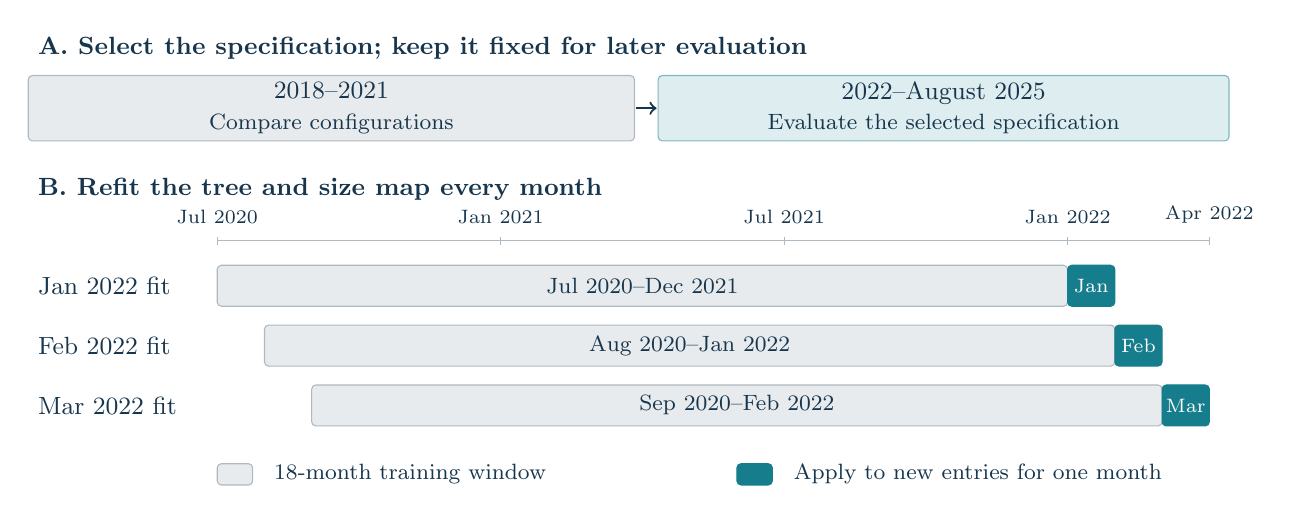
\begin{tikzpicture}[x=1cm,y=1cm,
 every node/.style={font=\small,text=navy},
 train/.style={fill=navy!10,draw=navy!35,rounded corners=1.5pt},
 apply/.style={fill=teal,draw=teal,rounded corners=1.5pt}]
\node[anchor=west,font=\small\bfseries] at (0,0)
 {A. Select the specification; keep it fixed for later evaluation};
\draw[train] (0,-1.18) rectangle (7.7,-0.35);
\node[align=center] at (3.85,-0.765)
 {2018--2021\\\footnotesize Compare configurations};
\draw[fill=teal!14,draw=teal!55,rounded corners=1.5pt]
 (8,-1.18) rectangle (15.25,-0.35);
\node[align=center] at (11.625,-0.765)
 {2022--August 2025\\\footnotesize Evaluate the selected specification};
\draw[->,draw=navy,thick] (7.72,-0.765) -- (7.98,-0.765);
\node[anchor=west,font=\small\bfseries] at (0,-1.8)
 {B. Refit the tree and size map every month};
\draw[draw=navy!35] (2.4,-2.45) -- (15,-2.45);
\foreach \x/\label in {2.4/Jul 2020,6/Jan 2021,9.6/Jul 2021,13.2/Jan 2022,15/Apr 2022}{
 \draw[draw=navy!35] (\x,-2.4) -- (\x,-2.5);
 \node[font=\scriptsize,anchor=south] at (\x,-2.35) {\label};
}
\node[anchor=west] at (0,-3.02) {Jan 2022 fit};
\draw[train] (2.4,-3.28) rectangle (13.2,-2.76);
\node[font=\footnotesize] at (7.8,-3.02) {Jul 2020--Dec 2021};
\draw[apply] (13.2,-3.28) rectangle (13.8,-2.76);
\node[text=white,font=\scriptsize] at (13.5,-3.02) {Jan};
\node[anchor=west] at (0,-3.78) {Feb 2022 fit};
\draw[train] (3,-4.04) rectangle (13.8,-3.52);
\node[font=\footnotesize] at (8.4,-3.78) {Aug 2020--Jan 2022};
\draw[apply] (13.8,-4.04) rectangle (14.4,-3.52);
\node[text=white,font=\scriptsize] at (14.1,-3.78) {Feb};
\node[anchor=west] at (0,-4.54) {Mar 2022 fit};
\draw[train] (3.6,-4.8) rectangle (14.4,-4.28);
\node[font=\footnotesize] at (9,-4.54) {Sep 2020--Feb 2022};
\draw[apply] (14.4,-4.8) rectangle (15,-4.28);
\node[text=white,font=\scriptsize] at (14.7,-4.54) {Mar};
\draw[train] (2.4,-5.55) rectangle (2.85,-5.28);
\node[anchor=west,font=\footnotesize] at (3,-5.415) {18-month training window};
\draw[apply] (9,-5.55) rectangle (9.45,-5.28);
\node[anchor=west,font=\footnotesize] at (9.6,-5.415) {Apply to new entries for one month};
\end{tikzpicture}
\caption{Two decisions, one historical dataset. The upper panel selects the
27-input, 18-month, 50/75/100\% specification using earlier performance.
The lower panel illustrates monthly refitting during evaluation. A training
example is included only if its signal date falls within the window and its
trade outcome is completed before that month's fit.}
\label{fig:rolling}
\end{figure}

We retain the configuration with the highest annualized daily excess Sharpe
on 2018--2021 among 33 existing configurations spanning training-history,
feature and sizing-action choices. The selected configuration uses 27 inputs,
an 18-month window and 50/75/100\% actions. Candidate identifiers break score ties; its selection score is 0.575 in a
\money{345 million} research account. This configuration is then replayed at
\money{10 million}; the account assumptions are summarized in
Appendix~\ref{app:implementation}.

Each monthly fit uses candidates that passed the entry screens on their signal
dates, have valid simulated outcomes, and finished before fitting. These
examples need not have been accepted by the funded account. Only signal dates
within the preceding 18 months enter the fit. Tree fitting and CEM use this
same sample; the wider candidate history supplies the profitability screens.

The later comparison runs from 3 January 2022 to 29 August 2025. The model
specification stays fixed while monthly refitting continues: a completed March
trade can inform an April fit, but an unfinished outcome cannot. New signals
stop on 30 June 2025. All accounts continue from 2018 with their own accumulated
cash and holdings; the 2022 boundary is a reporting split, not an account reset.

Later history had already been examined during strategy development. Monthly
fits respect time order, but this period is not independent of earlier choices
of contracts, screens and universe. Training also uses \money{0.65} commission
per option contract, compared with \money{0.03} for every policy in final
evaluation. We therefore interpret the comparison as historical evidence.

We report annualized Sharpe of daily returns above the cash benchmark, profit
above cash and cash-relative drawdown. Appendix~\ref{app:metrics} defines
these metrics and the opening portfolios at the reporting boundary.

\clearpage
\subsection{Learning an entry size: decision tree and CEM}
The opportunity rule fixes the pair, direction and contracts. We learn only
the entry size: 50\%, 75\% or 100\% of a reference budget of \money{450} vega
per IV point on each leg, scaled by current account equity relative to its
initial equity. Opportunities differ in their historical outcomes,
so the learner groups them and assigns a common size to each group
(Figure~\ref{fig:tree-cem}).

Each monthly regression tree receives 27 inputs: 15 numerical characteristics
and 12 availability flags, covering relative IV, trailing realized variance,
relatedness, maturity, the CBOE Volatility Index (VIX), costs and completed
profitability. Appendix~\ref{app:features} defines the inputs. It learns splits using historical
full-size profit above cash as its target, splitting to reduce squared
prediction error \cite{tree}. Each of its up to eight leaves is
a state. The cross-entropy method (CEM) \cite{cem} then chooses one size for each state.

\begin{figure}[H]
\centering
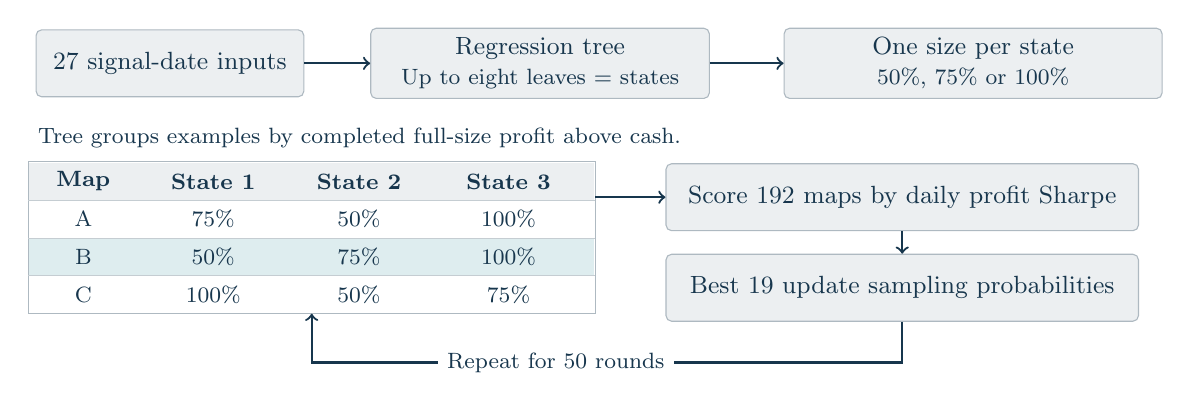
\begin{tikzpicture}[x=1cm,y=1cm,
 every node/.style={font=\small,text=navy},
 box/.style={draw=navy!35,fill=navy!8,rounded corners=2pt},
 flow/.style={->,draw=navy,thick}]
\node[box,align=center,minimum width=3.4cm,minimum height=0.85cm] (inputs) at (1.8,0)
 {27 signal-date inputs};
\node[box,align=center,minimum width=4.3cm,minimum height=0.85cm] (tree) at (6.5,0)
 {Regression tree\\\footnotesize Up to eight leaves = states};
\node[box,align=center,minimum width=4.8cm,minimum height=0.85cm] (map) at (12,0)
 {One size per state\\\footnotesize 50\%, 75\% or 100\%};
\draw[flow] (inputs)--(tree);\draw[flow] (tree)--(map);
\node[anchor=west,font=\footnotesize] at (0,-0.95)
 {Tree groups examples by completed full-size profit above cash.};
\draw[draw=navy!35] (0,-1.25) rectangle (7.2,-3.18);
\fill[navy!8] (0.01,-1.74) rectangle (7.19,-1.26);
\fill[teal!14] (0.01,-2.70) rectangle (7.19,-2.22);
\foreach \y in {-1.74,-2.22,-2.70}{\draw[draw=navy!25] (0,\y)--(7.2,\y);}
\foreach \x/\label in {0.7/Map,2.35/State 1,4.2/State 2,6.1/State 3}{
 \node[font=\footnotesize\bfseries] at (\x,-1.5){\label};}
\foreach \y/\name/\one/\two/\three in {-1.98/A/75/50/100,-2.46/B/50/75/100,-2.94/C/100/50/75}{
 \node[font=\footnotesize] at (0.7,\y){\name};
 \node[font=\footnotesize] at (2.35,\y){\one\%};
 \node[font=\footnotesize] at (4.2,\y){\two\%};
 \node[font=\footnotesize] at (6.1,\y){\three\%};}
\node[box,align=center,minimum width=6cm,minimum height=0.85cm] (score) at (11.1,-1.7)
 {Score 192 maps by daily profit Sharpe};
\node[box,align=center,minimum width=6cm,minimum height=0.85cm] (update) at (11.1,-2.85)
 {Best 19 update sampling probabilities};
\draw[flow] (7.2,-1.7)--(score);\draw[flow] (score)--(update);
\draw[flow] (update.south)--(11.1,-3.8)--(3.6,-3.8)--(3.6,-3.18);
\node[fill=white,font=\footnotesize] at (6.7,-3.8){Repeat for 50 rounds};
\end{tikzpicture}
\caption{Tree partitioning followed by CEM sizing search. The three-state
assignments illustrate candidate maps; actual trees have up to eight states.
The retained map applies to the next month's new proposals.}
\label{fig:tree-cem}
\end{figure}

\textbf{How CEM scores a size map}

A map $\boldsymbol m$ assigns size $a_\ell\in\{0.50,0.75,1.00\}$ to tree
state $\ell$. For completed example $i$, $x_i$ is its input vector and
$\ell(x_i)$ its state. Let $p_{i,d}(a)$ be profit above cash on trading day $d$
at size $a$. Each size uses its own rounded contracts and standalone cash
and hedge flows, rather than scaling the full-size outcome. A common stored
normalization cancels from the score. Sum paths and calculate
\[
g_d(\boldsymbol m)=\sum_i p_{i,d}\!\left(a_{\ell(x_i)}\right),\qquad
\widehat S_{\mathrm{train}}(\boldsymbol m)=\sqrt{252}\,
\frac{\overline{g(\boldsymbol m)}}{s_{g(\boldsymbol m)}}.
\]
Here $g_d$ is combined daily profit; the numerator and denominator are its
sample mean and standard deviation. The factor $\sqrt{252}$ annualizes using
252 trading days. The calendar retains overlapping trades and zero-profit
sessions. This standalone-profit training score differs from funded-account
Sharpe based on percentage returns and joint admission.

CEM updates size probabilities toward the best 19 of 192 maps, repeating for
50 rounds. Constant maps and the best map found so far are retained as anchors.
A new proposal receives its tree state's requested size, subject to account
admission. The search does not establish a global optimum.

\clearpage
\section{Benchmark and learned-sizing results}
\subsection{Does learned entry sizing improve the benchmark?}
We compare the tree/CEM policy with constant requests of 50\%, 75\% and 100\%
of the same reference budget. Each policy receives the same proposals and
keeps the proposed direction and contracts.

Figure~\ref{fig:performance} shows when profit above cash accumulates. Most of
the learner's final lead develops during 2022; both policies lose ground
during 2024.
\begin{figure}[H]
\centering
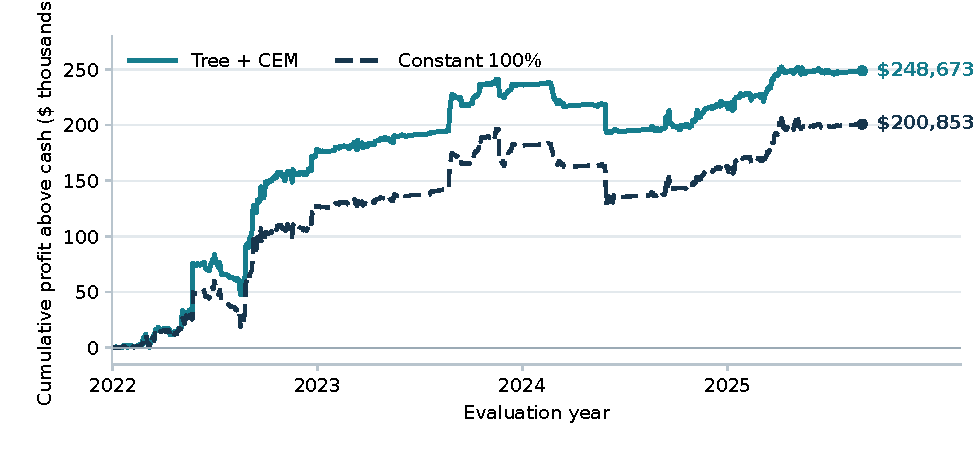
\includegraphics[width=\textwidth]{performance_above_cash.pdf}
\caption{Cumulative profit above cash, 3 January 2022--29 August 2025.
Curves are rebased at the 31 December 2021 close; the books retain carried
positions. Endpoints match Table~\ref{tab:main}. The paired 95\% interval for
the Sharpe gain, $[-0.103,0.424]$, includes zero.}
\label{fig:performance}
\end{figure}

Under the same proposals and funded-account rules, constant full sizing earns
later excess Sharpe of 1.055 and profit above cash of \money{200,853}, compared
with 1.263 and \money{248,673} for the learner (Table~\ref{tab:main}). The
observed gain is 0.208 Sharpe and approximately \money{47,800} additional
profit. This portfolio-policy comparison includes changes in which proposals
the account admits: 110 entries for the learner versus 75 for constant full sizing.
\begin{table}[htbp]
\centering\small
\begin{tabular}{lrrrrr}
\toprule
Policy & Earlier & Later & Later & Profit above & Relative\\
 & Sharpe & Sharpe & entries & cash (\$) & drawdown (\%)\\
\midrule
Constant 50\% & 0.437 & 1.007 & 151 & 204,913 & 0.735\\
Constant 75\% & 0.449 & 0.944 & 104 & 195,021 & 0.748\\
Constant 100\% & 0.478 & 1.055 & 75 & 200,853 & 0.646\\
Tree + CEM & 0.573 & 1.263 & 110 & 248,673 & 0.495\\
\bottomrule
\end{tabular}
\caption{Earlier: 2018--2021 replay at \money{10 million}; later:
January 2022--August 2025. Entries, profit and maximum cash-relative drawdown
refer to the later period. Earlier scores are \money{10 million} replay
scores, not the \money{345 million} configuration-selection scores.}
\label{tab:main}
\end{table}

The paired circular-block bootstrap, using 126-session blocks and
1,000 replications, gives a 95\% interval of $[-0.103,0.424]$ for the Sharpe gain.
It includes zero and omits search adjustment. The observed gain therefore does
not establish a repeatable sizing improvement. It also does not isolate gains
from sizing trades common to both policies.

The account earns annualized total return of 4.667\%, while annualized growth
relative to an all-cash account is 0.530\%. Most total account growth therefore
comes from cash interest. Trading is active---110 new entries---but its net
contribution above cash is modest: \money{248,673} over the later period.
Average reserve is 2.44\% of equity and peak reserve 15.77\%. Smaller requested
sizes can pass stress and pair limits that reject full-size proposals, even
when average account reserve is low. We use excess
Sharpe and profit above cash to assess the strategy's added value, rather than
attributing the full 4.667\% account return to trading.

\subsection{How does performance vary across years?}
Table~\ref{tab:annual} breaks the learner's later performance into calendar
periods. Its strongest annual cash-relative performance occurs in 2022,
which also accounts for 66 of the 110 later entries. In 2024, the account earns
a positive total return but loses relative to cash. The partial 2025 period
is positive above cash again. Together with Figure~\ref{fig:performance},
these results show that the aggregate profit reflects uneven performance
across years.
\begin{table}[H]
\centering\small
\begin{tabular}{lrrr@{\hspace{2em}}r}
\toprule
Year & Account return (\%) & Above cash (pp) & Excess Sharpe & Entries\\
\midrule
2022 & 3.470 & 1.673 & 2.458 & 66\\
2023 & 5.288 & 0.432 & 1.492 & 19\\
2024 & 5.104 & $-0.283$ & $-0.907$ & 11\\
2025 (partial) & 3.207 & 0.169 & 1.092 & 14\\
\bottomrule
\end{tabular}
\caption{Tree/CEM annual funded results; 2025 ends on 29 August.
Account and above-cash returns are unannualized for each displayed period,
including partial 2025. Above-cash figures are return differences in
percentage points; Sharpe is annualized.}
\label{tab:annual}
\end{table}

\section{Conclusion and limitations}
We compare constant sizing with a tree/CEM policy that learns entry sizes
from completed historical trades. Both policies use the same screened options
opportunities, hedging rules and funded-account constraints.

The constant-full rule earns positive historical profit above cash. Learned
sizing raises the funded point estimate, with a 0.208 Sharpe gain and
approximately \money{47,800} additional profit, but its gain interval includes
zero. It also admits more trades, 110 versus 75, under the same account rules.
Annual results vary, including a loss relative to cash in 2024. The evidence
supports a higher aggregate historical estimate for learned sizing, with
uncertainty about its repeatability.

The comparison uses previously inspected history and differs across training,
selection and evaluation in capital, costs and admission. Execution and option
exercise are simplified. These results establish neither repeatable learning
benefits nor live profitability or capacity. Most account growth is cash
interest; trading value is measured above cash.

\clearpage
\appendix
\small
\section{Signal and learning specification}
\label{app:implementation}
Choose the expiry closest to 30 days in the historical anchor selection, then
the put in that expiry nearest absolute delta 0.25, within 0.075. Ties favor
narrower spreads, higher open interest and lower contract identifier. Entry
requires standard 100-share contracts, positive noncrossed quotes, open
interest at least 100, width at most 25\% of midpoint and 7--55 days remaining.
The IV rank includes the signal close; relatedness is fixed monthly from the
prior 126 sessions. Profitability memory uses completion dates, not entry dates.

Admission stress sums each name's worst modeled option-plus-hedge loss across
spot shocks of $-20/0/+20$\% and IV shocks of $-10/0/+10$ percentage points,
without credit for pair correlation. Stress loss is capped at 5\% of budget;
reserve (gross option premium plus half netted hedge notional) at 80\%, hedge
notional at twice budget and gross vega at \money{20,000} per IV point per
\money{1 million}. Global checks use account equity; pair checks use
\money{1 million} scaled by current/initial account equity. Proposals are
processed in pair-identifier order. These are research limits, not broker margin.
Corporate events or unsupported declared distributions exit affected pairs;
missing entry quotes reject proposals, while held marks may use last-known IV
with current spot, rates and known dividends. Expiry is cash-settled with a
European valuation approximation; market impact, early assignment and forced
liquidation are not fully modeled.

The tree has up to eight leaves, with minimum leaf count one eighth of its
training sample rounded down, bounded between 8 and 63. Fewer than 16 examples
use full sizing. CEM begins uniformly each month and mixes 30\% current
probability with 70\% elite frequency, multiplies by 0.97 and adds 0.03 equally
across the three actions. The random seed is 2026.

\subsection{Inputs available at the signal date}
\label{app:features}
The model uses the following 15 numerical inputs. Proposed-direction quantities
are oriented as long leg minus short leg. IV and volatility levels are decimal
annualized values. Trailing realized variance is 252 times mean squared daily
simple returns over the latest 20 listed trading sessions, with at least 10
observations, including the signal-close return. Returns generally exclude dividends; adjusted-close percentage changes
provide the fallback series.

\begin{center}
\small
\begin{tabular}{p{0.32\textwidth}p{0.61\textwidth}}
\toprule
Input & Definition\\
\midrule
Mean IV & Mean of the two selected-contract IVs.\\
Oriented IV gap & Long-minus-short IV divided by mean IV.\\
Rank strength & Twice the absolute distance of the IV-gap percentile from 0.5.\\
Oriented variance-premium gap & Long-minus-short difference in IV squared minus trailing realized variance, divided by mean IV squared.\\
Mean RV & Mean of the square roots of the two trailing realized variances.\\
Beta; correlation & Two inputs: 126-session A-on-B beta and correlation, fixed at monthly formation.\\
Mean expiry; expiry gap & Two inputs: mean calendar days to expiry and long-minus-short expiry days.\\
Commission in IV points & Sum across legs of \money{0.65} divided by each contract's dollar vega per IV point.\\
VIX & Most recent strictly prior VIX close divided by 100.\\
91-day profit; count & Two inputs: completed full-size profit per initial vega averaged over the trailing 91 calendar days and the number of completed outcomes. The profit input is divided by 100 as a fixed scale.\\
365-day profit; count & Two inputs: the same measurements over 365 calendar days.\\
\bottomrule
\end{tabular}
\end{center}
The first three inputs are core fields. Each of the other 12 has a binary
availability flag, giving 27 inputs in total. Nonfinite optional values receive
zero and flag zero; observed values have flag one. Profit features use only outcomes completed before the signal date;
future returns and profits enter outcomes, not inputs.

\clearpage
\section{Performance definitions and evidence}
\label{app:metrics}
Let $N_t$ be account equity and $K_t$ all-cash benchmark wealth at close $t$.
Both start at \money{10 million} in January 2018. The benchmark compounds the
previous available WRDS zero-curve rate nearest 30 days over calendar days
using a 365-day year. Daily excess return and annualized Sharpe are
\[
e_t=\left(\frac{N_t}{N_{t-1}}-1\right)
-\left(\frac{K_t}{K_{t-1}}-1\right),\qquad
\widehat S=\sqrt{252}\,\bar e/s_e.
\]
Here $\bar e$ and $s_e$ are the sample mean and standard deviation of daily
excess returns; 252 is assumed trading days per year. For a reporting period
with preceding close $0$ and final close $T$, dollar profit above cash is
$(N_T-K_T)-(N_0-K_0)$. Set $Q_t=N_t/K_t$: annualized relative growth is
$(Q_T/Q_0)^{1/Y}-1$, where $Y$ is elapsed days divided by 365.25.
Cash-relative drawdown is the largest percentage decline in $Q_t$ from its
running peak within that period, including close $0$.

Annual-table account return is $N_T/N_0-1$; above-cash percentage points
subtract benchmark return $K_T/K_0-1$. Period returns are unannualized,
including partial 2025; Sharpe remains annualized. At the 31 December 2021
boundary, learner and constant-full equity are \money{10.568 million} and
\money{10.581 million}, with four and three open trades respectively.
Benchmark wealth is \money{10.510 million}. Chart curves subtract each policy's
opening dollar excess wealth; accounts and holdings are not reset.

The gain interval resamples the learner and constant-full daily excess returns
with identical indices: 1,000 samples concatenate randomly started 126-session
blocks, wrap at the series end and truncate to original length. Each sample
recalculates the Sharpe difference; endpoints are its 2.5th and 97.5th
percentiles. Fitted policies are fixed and research selection is unadjusted.

{\raggedright
\textbf{Evidence sources.} Results and implementation use repository snapshot
\href{https://github.com/kreitzz/rl-atm-vega-pairs/tree/688bc3909ba09be77af90df2d1c2696f316fedbe}{688bc39}.
The directory \path{reports/p25_validation_split} contains
\path{periods.csv}, \path{annual.csv}, \path{holdout_intervals.csv} and
\path{selection.json}. Figure~\ref{fig:performance} uses the selected account in
\path{data/p25_validation_split_experiment.zip} and the constant-full account
under \path{data/submission/artifacts/contracts/p25_capital_sensitivity}.
The complete 125-pair roster, candidate-date ranges and proposal counts are
retained in the companion \path{paper/pair_universe.csv}; ranges describe
recorded candidates, not continuous quote coverage or executed trading dates.
Inherited formation calendars and usable contracts condition the universe.
Vendor data retain their institutional license restrictions.\par}

\begin{thebibliography}{9}
\raggedright
\bibitem{ning} B.~Ning and K.~Lee (2024).
\emph{Advanced Statistical Arbitrage with Reinforcement Learning}.
arXiv:2403.12180v1. \url{https://arxiv.org/abs/2403.12180}.
\bibitem{cem} P.-T.~de Boer, D.~P.~Kroese, S.~Mannor and R.~Y.~Rubinstein (2005).
\emph{A Tutorial on the Cross-Entropy Method}.
Annals of Operations Research 134, 19--67.
\url{https://people.smp.uq.edu.au/DirkKroese/ps/aortut.pdf}.
\bibitem{tree} scikit-learn documentation. \emph{DecisionTreeRegressor}.
\url{https://scikit-learn.org/stable/modules/generated/sklearn.tree.DecisionTreeRegressor.html}.
\end{thebibliography}
\end{document}
